\section{Tuning}\label{sec:tuning}
In machine learning there is no default set of parameters or rule set which will
gaurantee optimal performance.
The only conclusive method to find optimal parameter values is to evaluate
each by comparison.
This can quickly lead to overfitting if the results are misinterpreted or
incorrectly measured.

The primary cause of overfitting is tuning on the entire dataset.
To reduce the chance of this, datasets should be split into development
and evaluation sets, on top of cross validation.
Although we don't do this here, we do use 10-times 10-fold cross validation as
described in Section~\ref{sec:acc_eval}.

The OOB error rate gives us an estimate of real-world performance, and we may
gain some insight into whether or not we are actaully gaining performance in
other metrics or overfitting by comparing this with the OOB error.\\

In order to confidently produce unbiased statistics, and ensure that tuning is
not guided to overfitting, validation curves should be computed.
These compare
the performance of the classifier on separate training and validation datasets.
This has not been done because we have not collected sufficient data to be able
to split it further, on top of the cross validation used.

We could also plot the learning rate, which shows the performance of the classifier
with a varying number of samples, allowing us to gauge whether adding more
samples will improve classification scores or not.
This has also not been done.


\subsection{Gridsearch}
The most basic form of parameter search is gridsearch.
A set of influential parameters are chosen, as well as a range of discrete
values to test.
Gridsearch then involves the exhaustive enumeration of all possible parameter
value combinations.

We test each combination using the usual evaluation mechanism with the following
search space:
\begin{itemize}
  \item Number of Estimators: 10, 35, 50, 75, 90, 100, 110, 250, 300, 500, 5000, 10000
  \item Max features: $sqrt(n)$, $log2(n)$, $0.33*n$
\end{itemize}

The effect of each parameter is described in Section~\ref{sec:param}.
We have not tested other parameters due to the time cost of doing so.


\subsubsection{Results}


The OOB error rate (Figure~\ref{fig:tuning_oob}) shows that the random forest is
predicted to achieve peak
performance with $0.33 * n. features$ at around 300 estimators, rising outside
the stable range of $]150,500[$.
The error rate plateaus at about 500 estimators for all max feature functions.

Accuracy (Figure~\ref{fig:tuning_acc}) and F1-score (Figure~\ref{fig:tuning_f1})
show that peak performance is achieved somewhere between $[75,300[$ estimators
for all max feature functions, peaking at 89\% accuracy for $0.33*n$.
This correlates with the global minimum OOB error at 300 estimators.

Both metrics quickly drop somewhere between $[300,500]$, where the random forest
is most likely beginning to overfit and lose generalisation.
After this point, as the number of trees increases, we observe overfitting as
accuracy, F1-score, and the OOB error rate increases.

Because the OOB error begins to stabalise at 100, it is likely that peak
real-world performance will lie within $[100,300[$ for most max feature functions.

Performance improvements are generally observed with the increase in max features.
The linear max features function shows a smoother response and better
performance overall.\\

Without a completely independent validation data set it is impossible to perform
an evaluation which is truly representative of real-world performance.

\begin{figure}[!htb]
  \centering
  \begin{subfigure}[b]{0.70\textwidth}
    \centering
    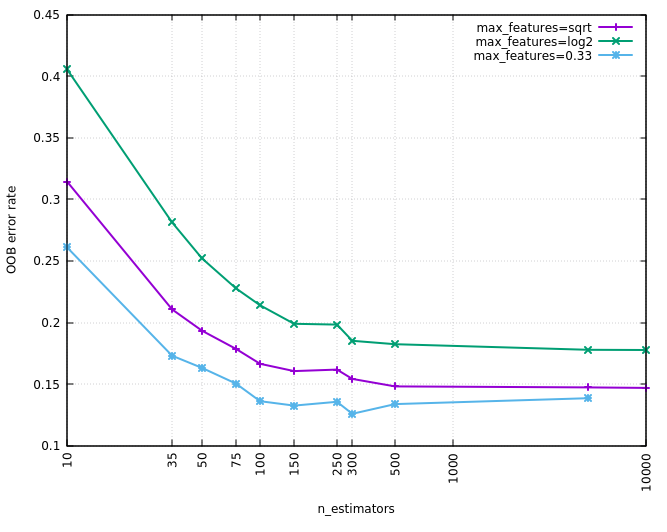
\includegraphics[width=1.0\textwidth]{plt_oob}
    \caption{OOB error}
    \label{fig:tuning_oob}
  \end{subfigure}\\
  \begin{subfigure}[b]{0.5\textwidth}
    \centering
    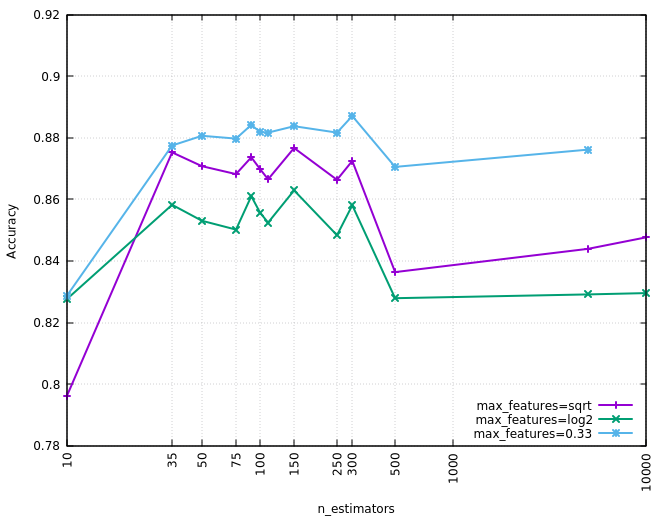
\includegraphics[width=1.0\textwidth]{plt_acc}
    \caption{Accuracy}
    \label{fig:tuning_acc}
  \end{subfigure}%
  \begin{subfigure}[b]{0.5\textwidth}
    \centering
    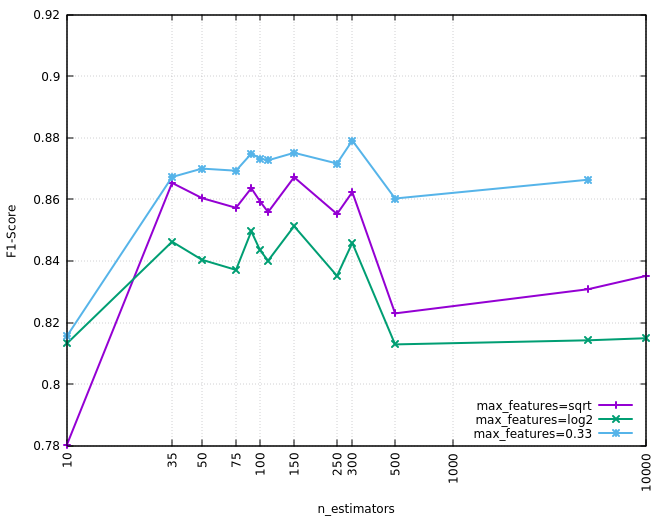
\includegraphics[width=1.0\textwidth]{plt_f1}
    \caption{F1-Score}
    \label{fig:tuning_f1}
  \end{subfigure}
%  \begin{subfigure}[b]{0.5\textwidth}
%    \centering
%    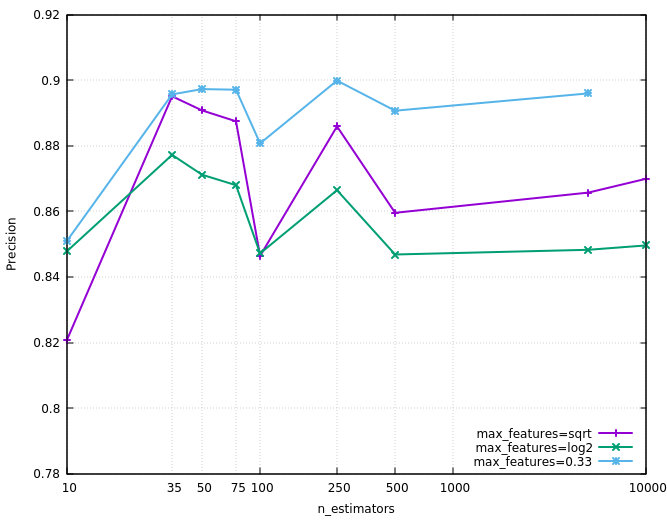
\includegraphics[width=1.0\textwidth]{plt_prc}
%    \caption{Precision}
%  \end{subfigure}%
%  \begin{subfigure}[b]{0.5\textwidth}
%    \centering
%    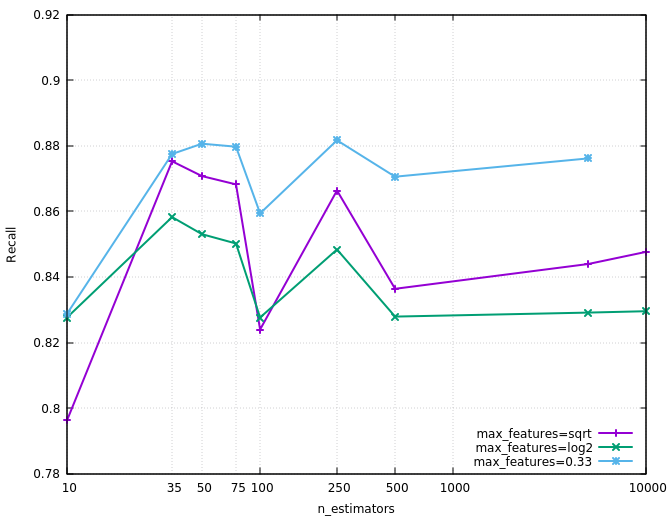
\includegraphics[width=1.0\textwidth]{plt_rec}
%    \caption{Recall}
%  \end{subfigure}
  \caption{Metrics over n. estimators for each max feature function}
  \label{fig:tuning}
\end{figure}
